\begin{flushright} {\tiny {\color{gray} python\_codes/fieldstone\_123/text.tex}} \end{flushright}

\lstinputlisting[language=bash,basicstyle=\small]{python_codes/fieldstone_123/keywords}

\begin{center}

\fbox{\textbf{\huge \color{teal} P}}
Code at \url{https://github.com/cedrict/fieldstone/tree/master/python_codes/fieldstone_123}
\end{center}

\par\noindent\rule{\textwidth}{0.4pt}

%%%%%%%%%%%%%%%%%%%%%%%%%%%%%%%%%%%%%%%%%%%%%%%%%%%%%%%%%%%%%%%%%%%%%%%%%%%%%%%%%%%%%%%%%%%%%%%%

%------------------------------
\subsubsection*{Love's problem (exp=1)}

The domain is a cuboid of size $L_x\times L_y \times L_z$ with $L_x=L_y=\SI{5}{\km}$
and $L_z=\SI{2.5}{\km}$. 
It is filled with a single elastic material characterised by $E=\SI{0.6e11}{\pascal}$ and $\nu=0.25$. 

We consider the elastic surface displacements generated by an 
applied pressure equivalent to $\SI{100}{\meter}$ 
water depth in a rectangular area $2a\times 2b = 2\times 1~\si{\km}$
as in \textcite{bebe04} (2004).
Because of the inherent symmetry of the problem we model only one quarter ('the top right')
of the problem.

\begin{center}
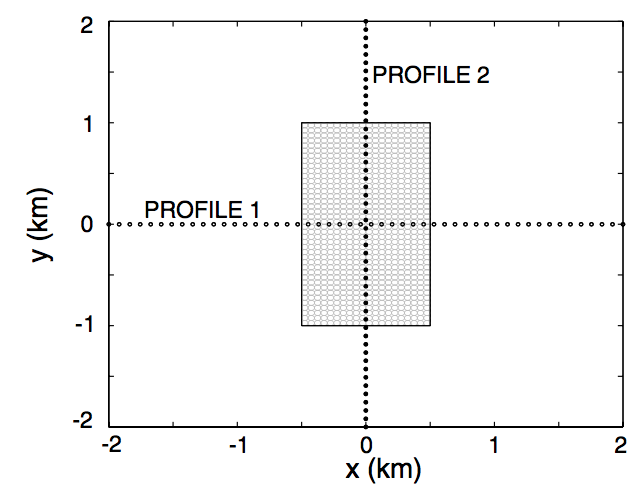
\includegraphics[width=6cm]{python_codes/fieldstone_123/images/fig1}\\
{\captionfont Note that we use a domain of different size.}
\end{center}

Boundary conditions are as follows: The analytical solution is prescribed on 
all sides and bottom while traction boundary conditions are prescribed on a 
rectangle of size $a\times b$. 
The analytical solution of this problem is is the {\pythonfile love.py} file.
$Q_1$ elements are used. 

\begin{center}
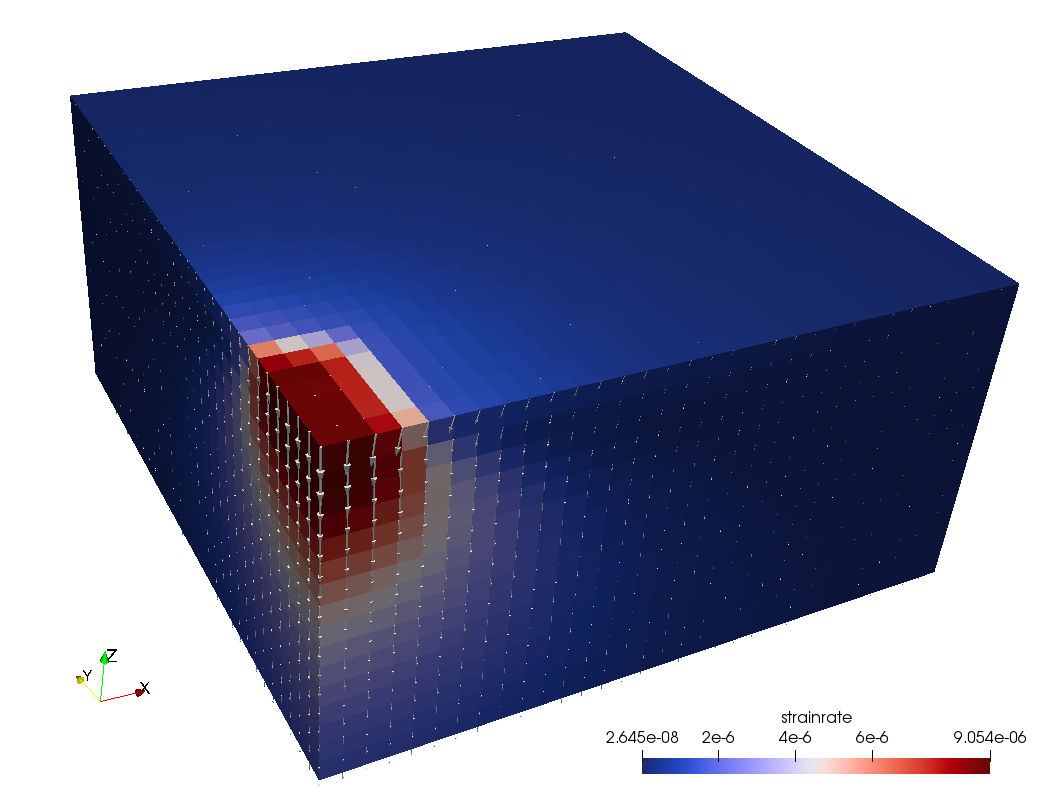
\includegraphics[width=8cm]{python_codes/fieldstone_123/results/exp1/disp} 
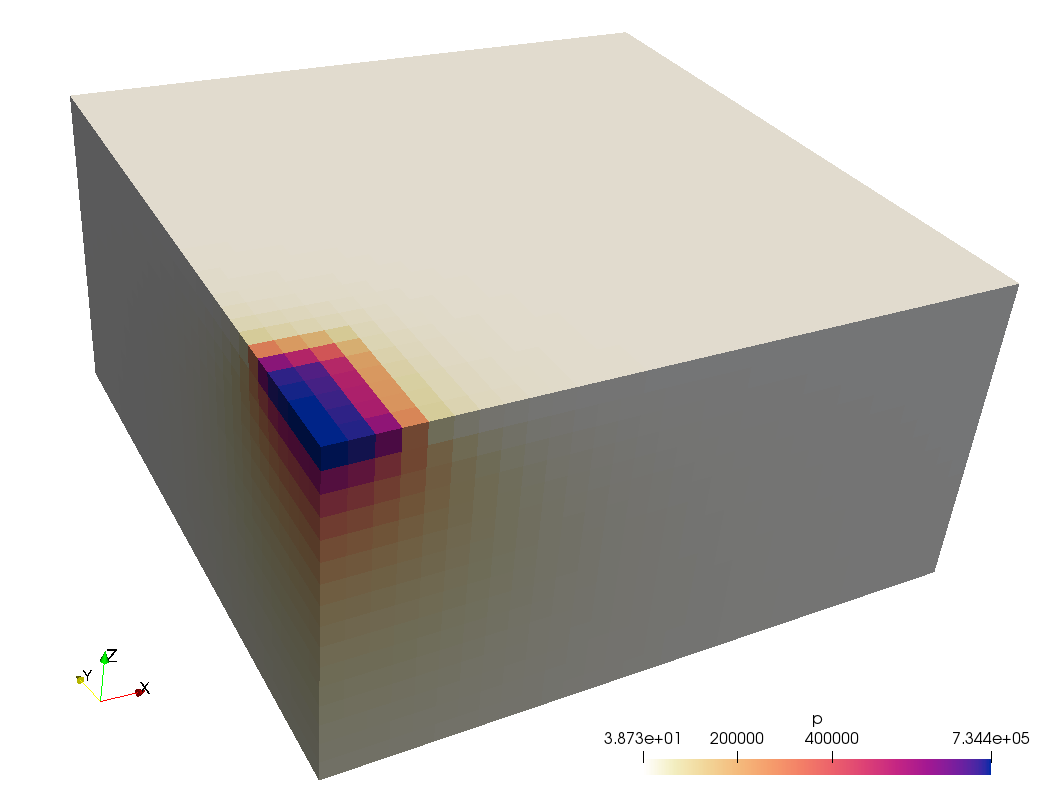
\includegraphics[width=8cm]{python_codes/fieldstone_123/results/exp1/press} \\
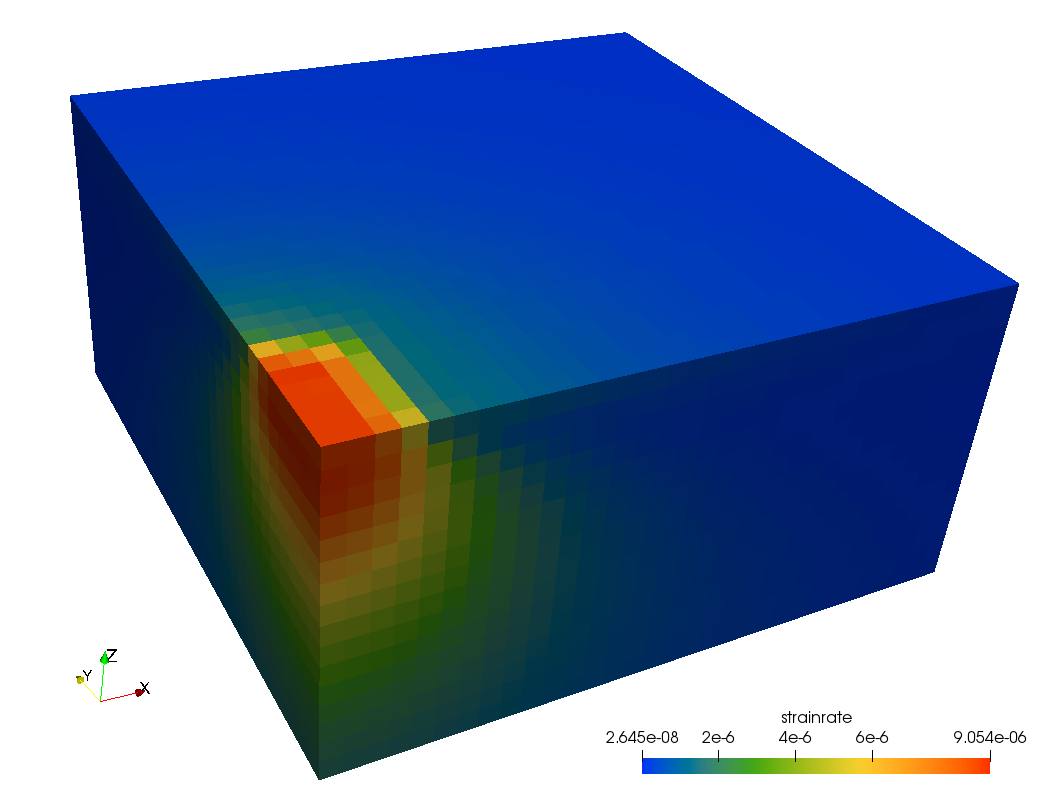
\includegraphics[width=8cm]{python_codes/fieldstone_123/results/exp1/sr} 
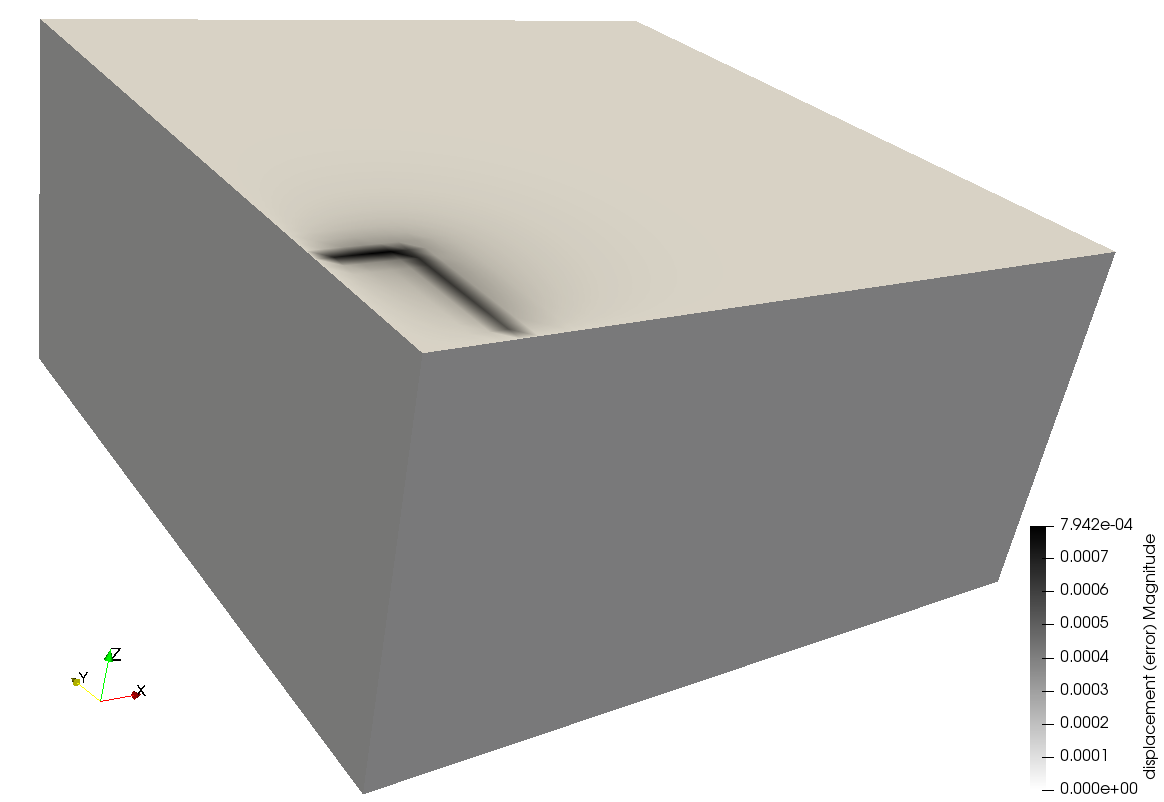
\includegraphics[width=8cm]{python_codes/fieldstone_123/results/exp1/error} \\
{\captionfont $32\times 32\times 32$ mesh}
\end{center} 


\begin{center}
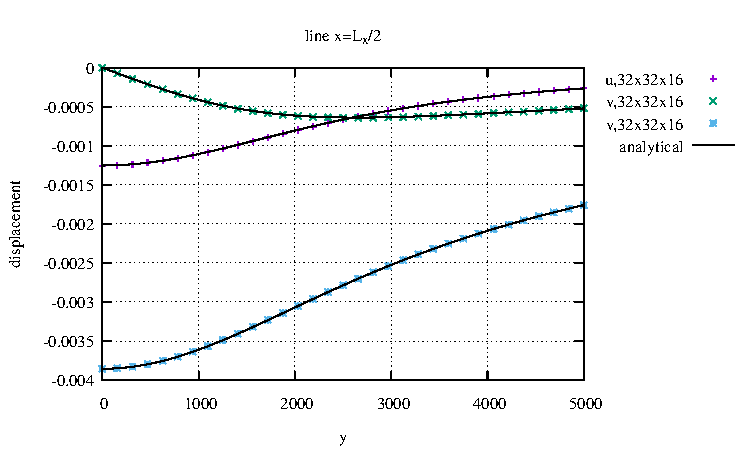
\includegraphics[width=8cm]{python_codes/fieldstone_123/results/exp1/xprofile.pdf} 
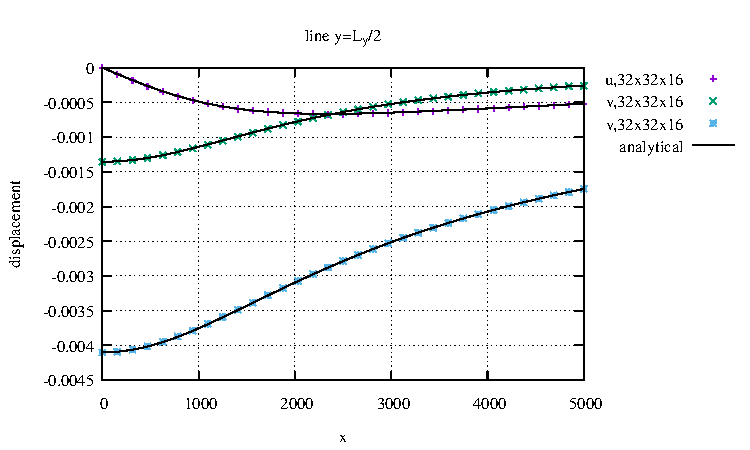
\includegraphics[width=8cm]{python_codes/fieldstone_123/results/exp1/yprofile.pdf} \\
{\captionfont Three components of the displacement vector $\vec{\upupsilon}$
on $x=L_x/2$ and $y=L_y/2$ lines.}
\end{center}

%----------------------------------
\subsubsection*{Boussinesq problem (exp=2)}





